\section{Harsh Zota}\label{harsh-zota}

\subsubsection{07700000128}\label{section}

\section{Distributed System Programming
Assignment-1}\label{distributed-system-programming-assignment-1}

\subsection{Project Summary}\label{project-summary}

This project involves the development of a basic HTTP server in C for a
distributed systems assignment. The server handles client connections,
processes HTTP GET requests, and serves static files, including HTML
pages (\texttt{index.html} and \texttt{info.html}), images, and videos.
The server supports external video links and direct access to images or
text files through URLs, while handling errors gracefully by serving
specific error pages (\texttt{400.html}, \texttt{403.html},
\texttt{404.html}, and \texttt{500.html}). Logging features are
implemented to track new connections, resource requests, permission
issues, and connection closures. The project demonstrates fundamental
concepts in socket programming, multithreading, and HTTP server
functionality.

\subsection{Project Structure}\label{project-structure}

\begin{figure}
\centering
\pandocbounded{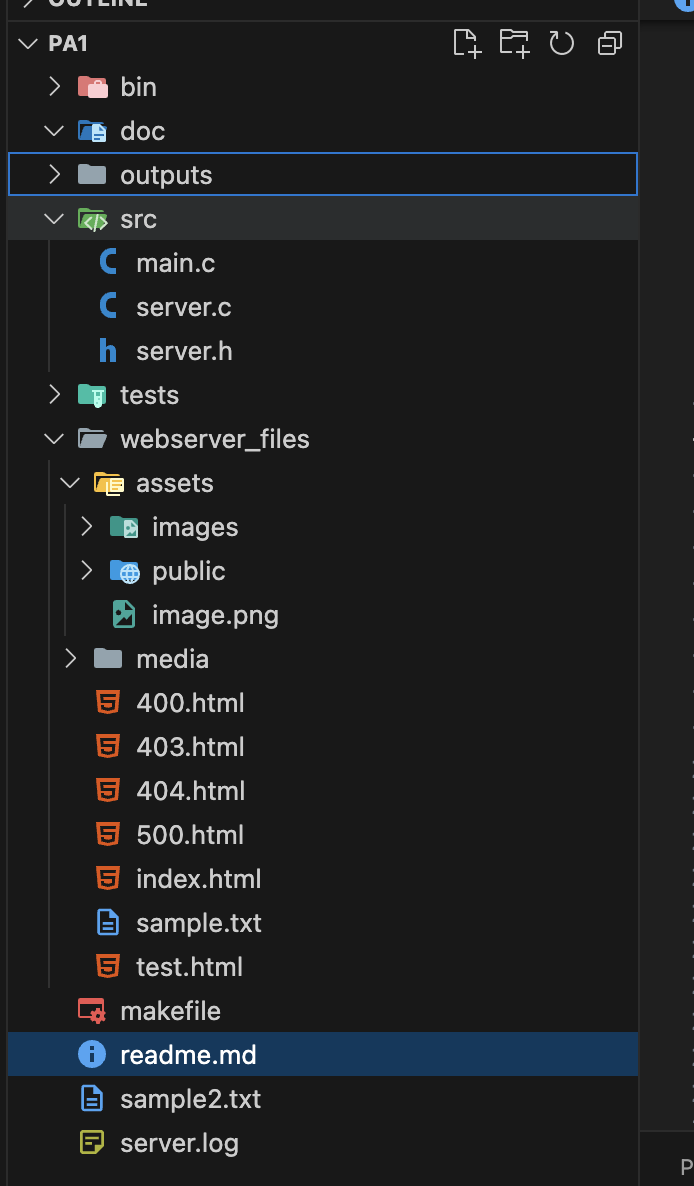
\includegraphics[keepaspectratio]{/outputs/files.png}}
\caption{Alt text}
\end{figure}

\subsection{Instructions to Run the
Program}\label{instructions-to-run-the-program}

\begin{enumerate}
\def\labelenumi{\arabic{enumi}.}
\item
  \textbf{Setup the Environment}:

  \begin{itemize}
  \tightlist
  \item
    Ensure you have \texttt{gcc} installed on your system.
  \item
    Navigate to the project directory containing the \texttt{src},
    \texttt{webserver\_files}, and other directories.
  \end{itemize}
\item
  \textbf{Compile the Server Code}:

\begin{Shaded}
\begin{Highlighting}[]
\FunctionTok{make}
\end{Highlighting}
\end{Shaded}

  This will compile the source files and generate the server executable.
\item
  \textbf{Run the Server}:

\begin{Shaded}
\begin{Highlighting}[]
\ExtensionTok{./bin/server}
\end{Highlighting}
\end{Shaded}

  The server will start listening on the specified port (e.g., 8000 or
  8888).
\item
  \textbf{Access the Server}:

  \begin{itemize}
  \tightlist
  \item
    Open your browser and visit \texttt{http://localhost:8888} to see
    the default page.
  \item
    Test other paths like \texttt{info.html}, image files, or text
    files.
  \end{itemize}
\item
  \textbf{Log Files}:

  \begin{itemize}
  \tightlist
  \item
    Logs are saved in \texttt{server.log} which captures connection
    events, file requests, errors, and other server-side activities.
  \end{itemize}
\end{enumerate}

\subsection{Images and Descriptions}\label{images-and-descriptions}

\subsubsection{1. Image of Logs}\label{image-of-logs}

\pandocbounded{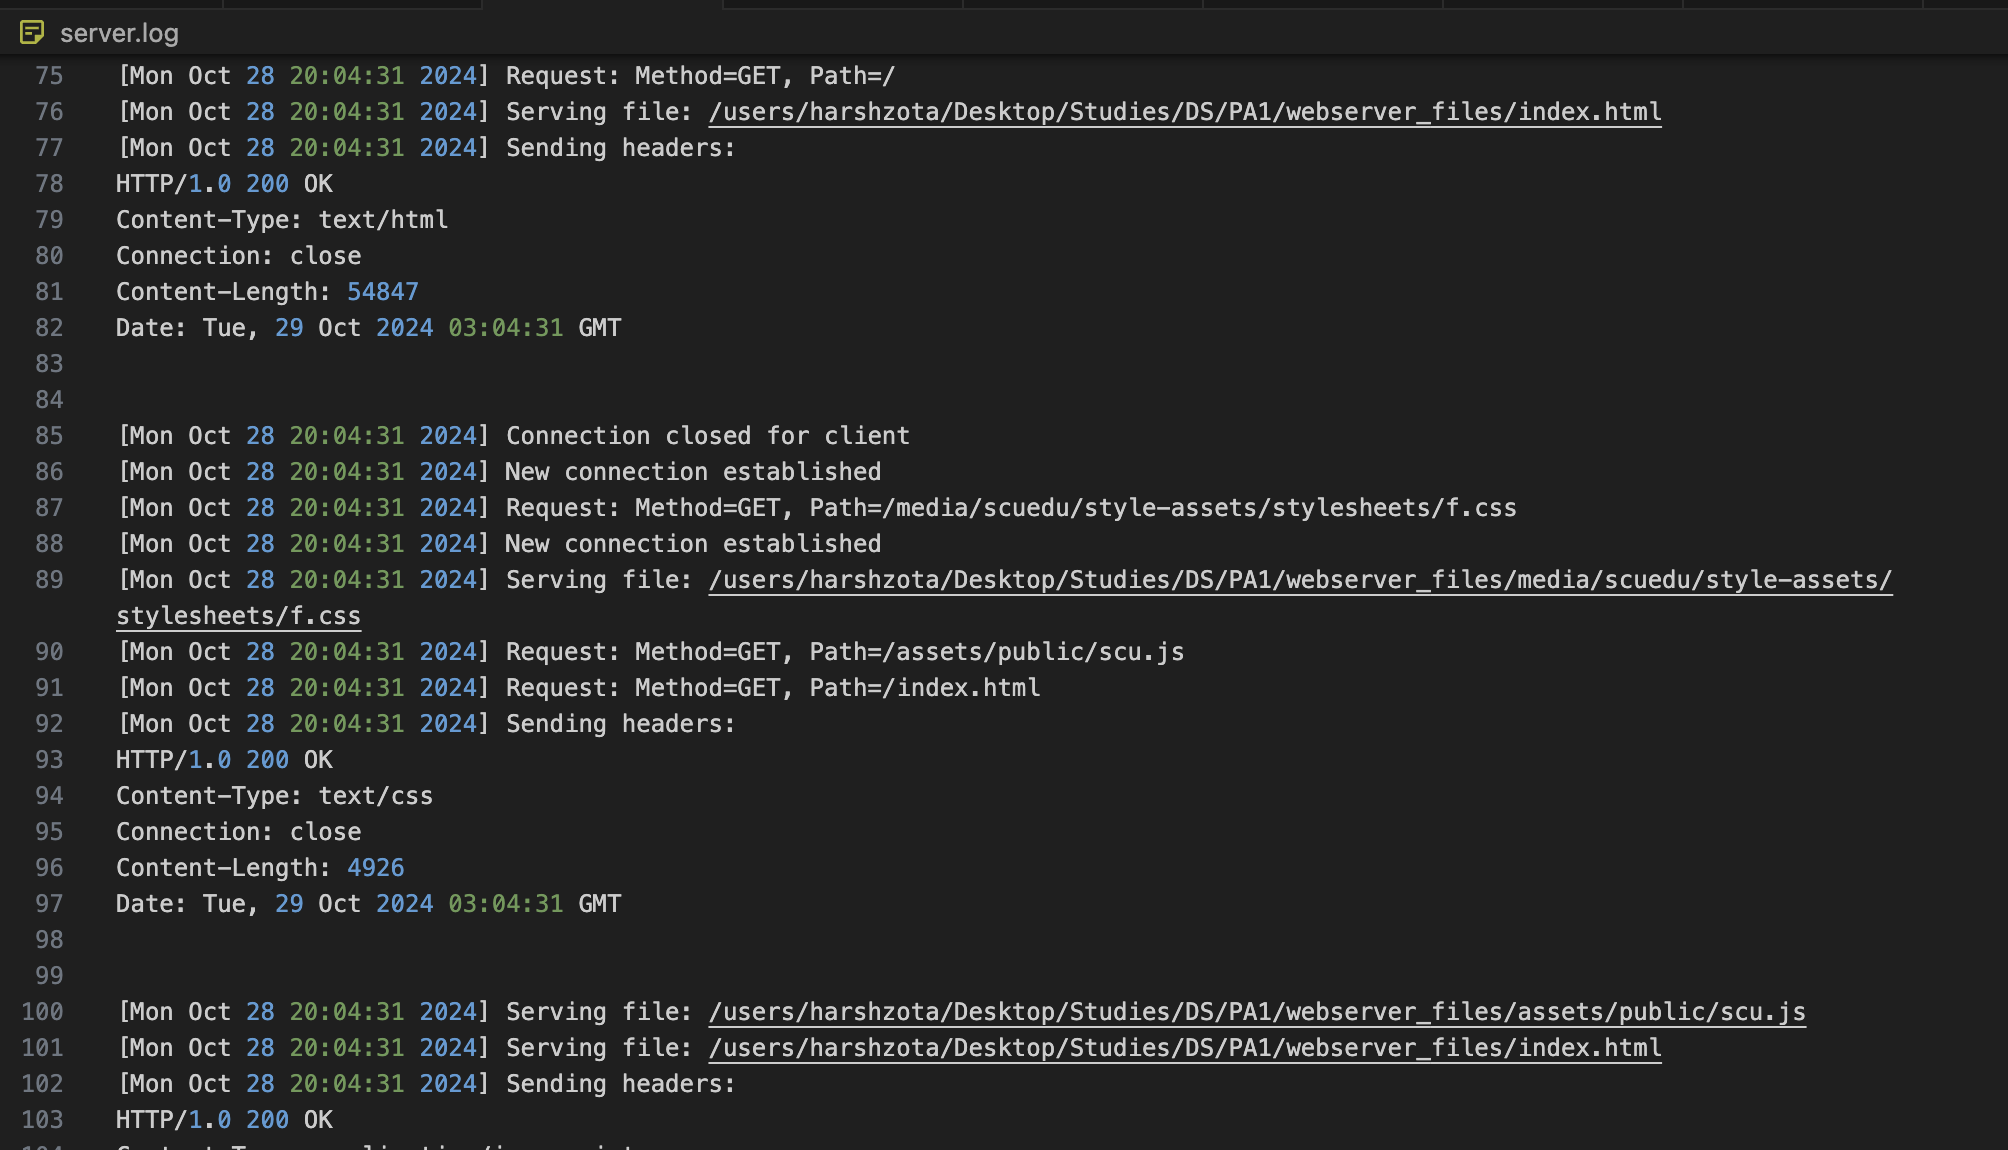
\includegraphics[keepaspectratio]{/outputs/logs1.png}}
\pandocbounded{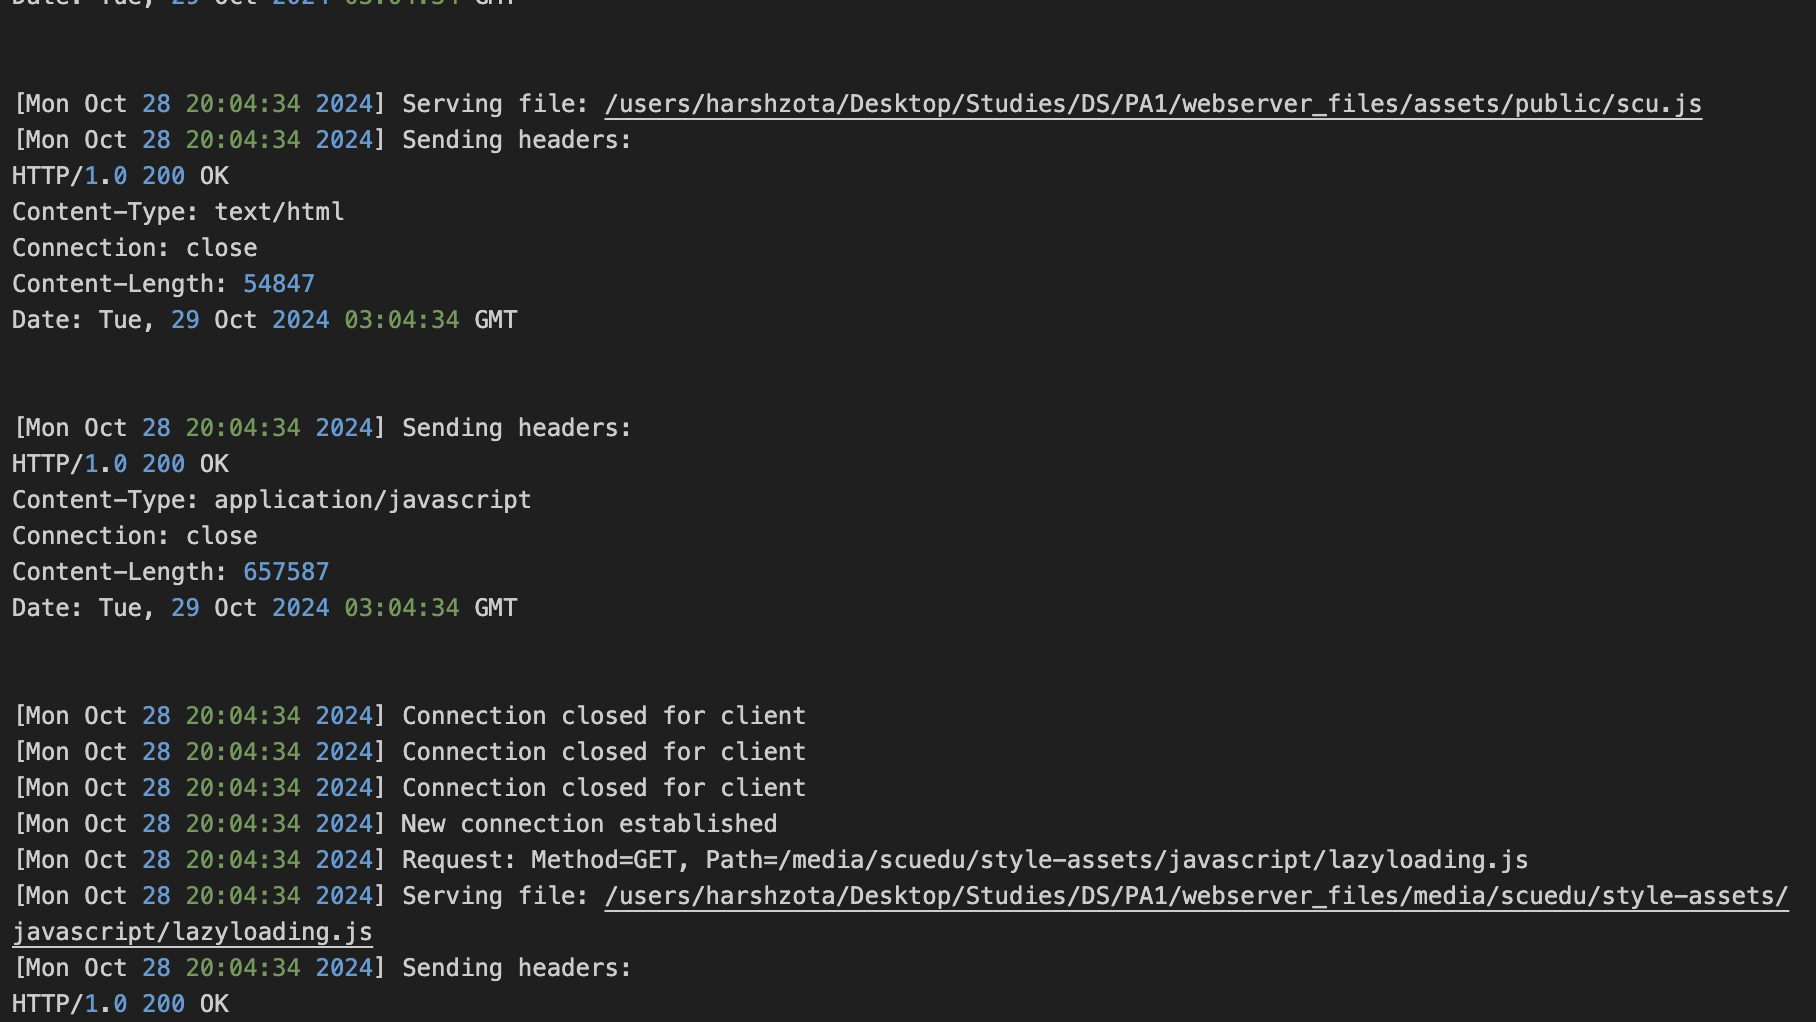
\includegraphics[keepaspectratio]{/outputs/logs2.png}} -
This image shows the content of the \texttt{server.log} file, which
records new connections, resource requests, and client disconnections,
including detailed timestamps.

\subsubsection{2. Image of Default Page}\label{image-of-default-page}

\pandocbounded{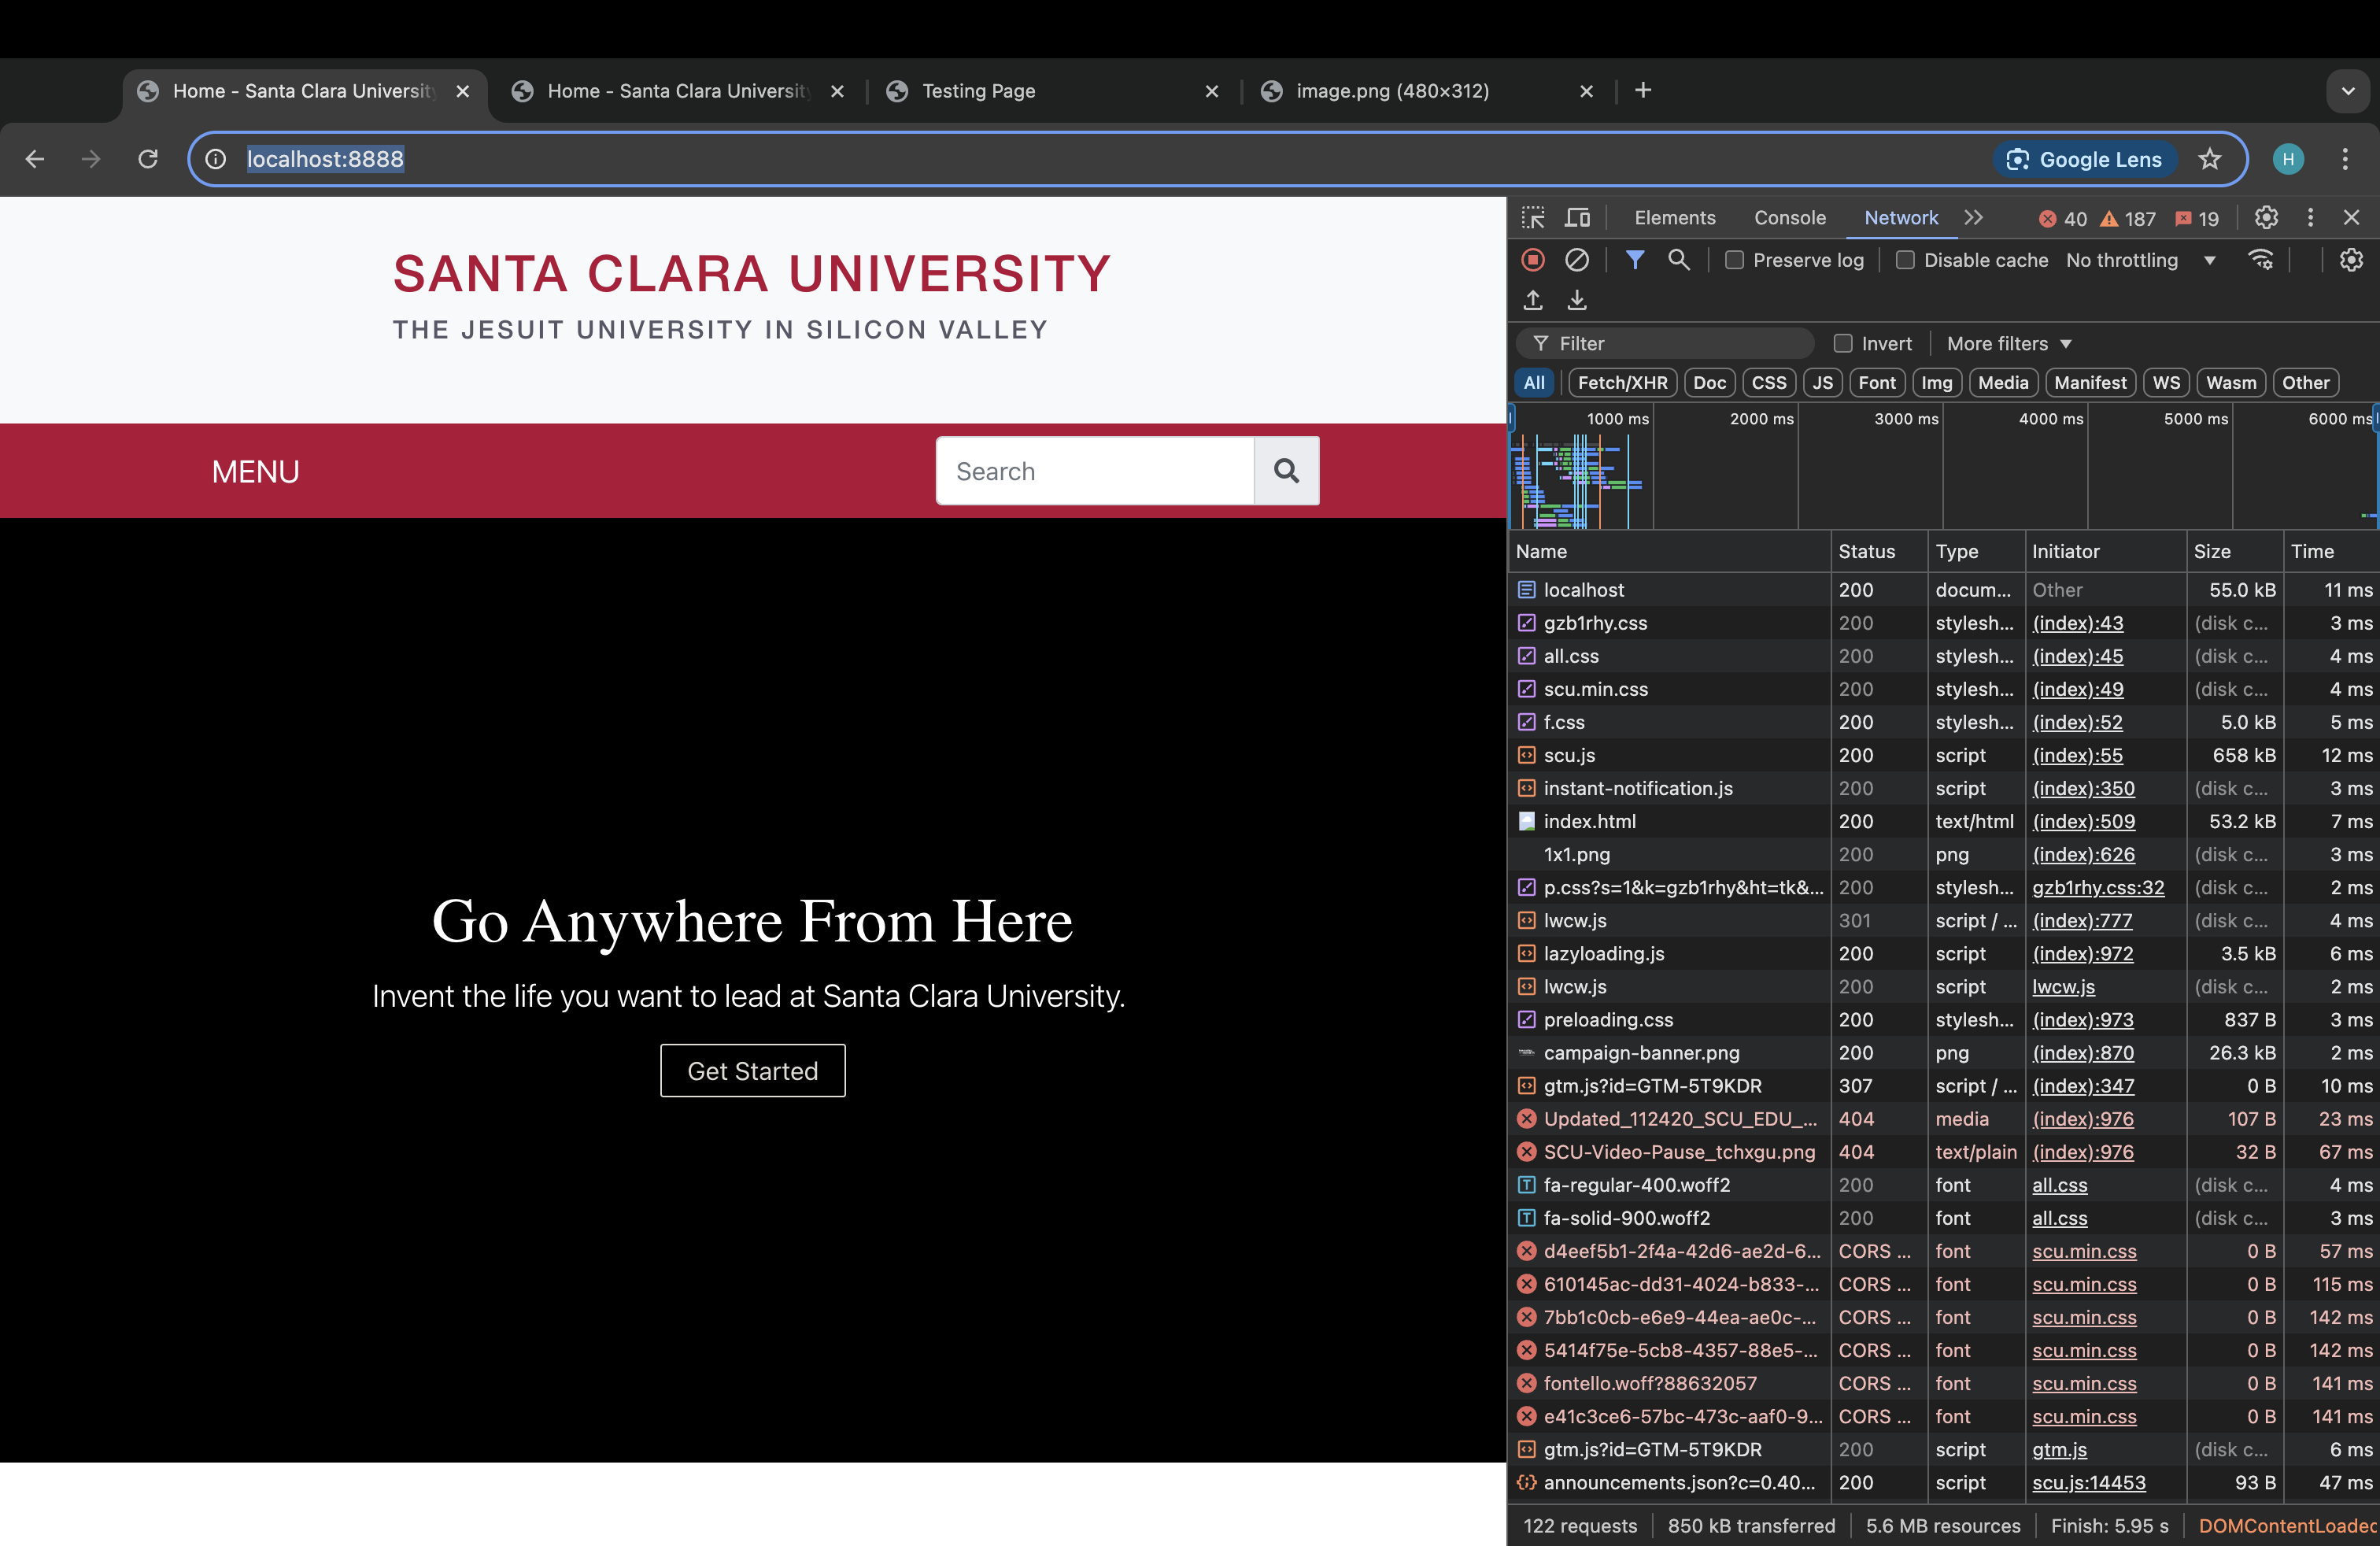
\includegraphics[keepaspectratio]{/outputs/default.png}}
- The default page (\texttt{index.html}) is served when the root URL is
accessed. It contains basic information about the project.

\subsubsection{\texorpdfstring{3. Image of \texttt{index.html}
Page}{3. Image of index.html Page}}\label{image-of-index.html-page}

\pandocbounded{
\includegraphics[keepaspectratio]{/outputs/index.png}} -
The \texttt{index.html} page served at the root directory is a simple
HTML page, including links and text describing Santa Clara University.

\subsubsection{\texorpdfstring{4. Image of \texttt{info.html}
Page}{4. Image of info.html Page}}\label{image-of-info.html-page}

\pandocbounded{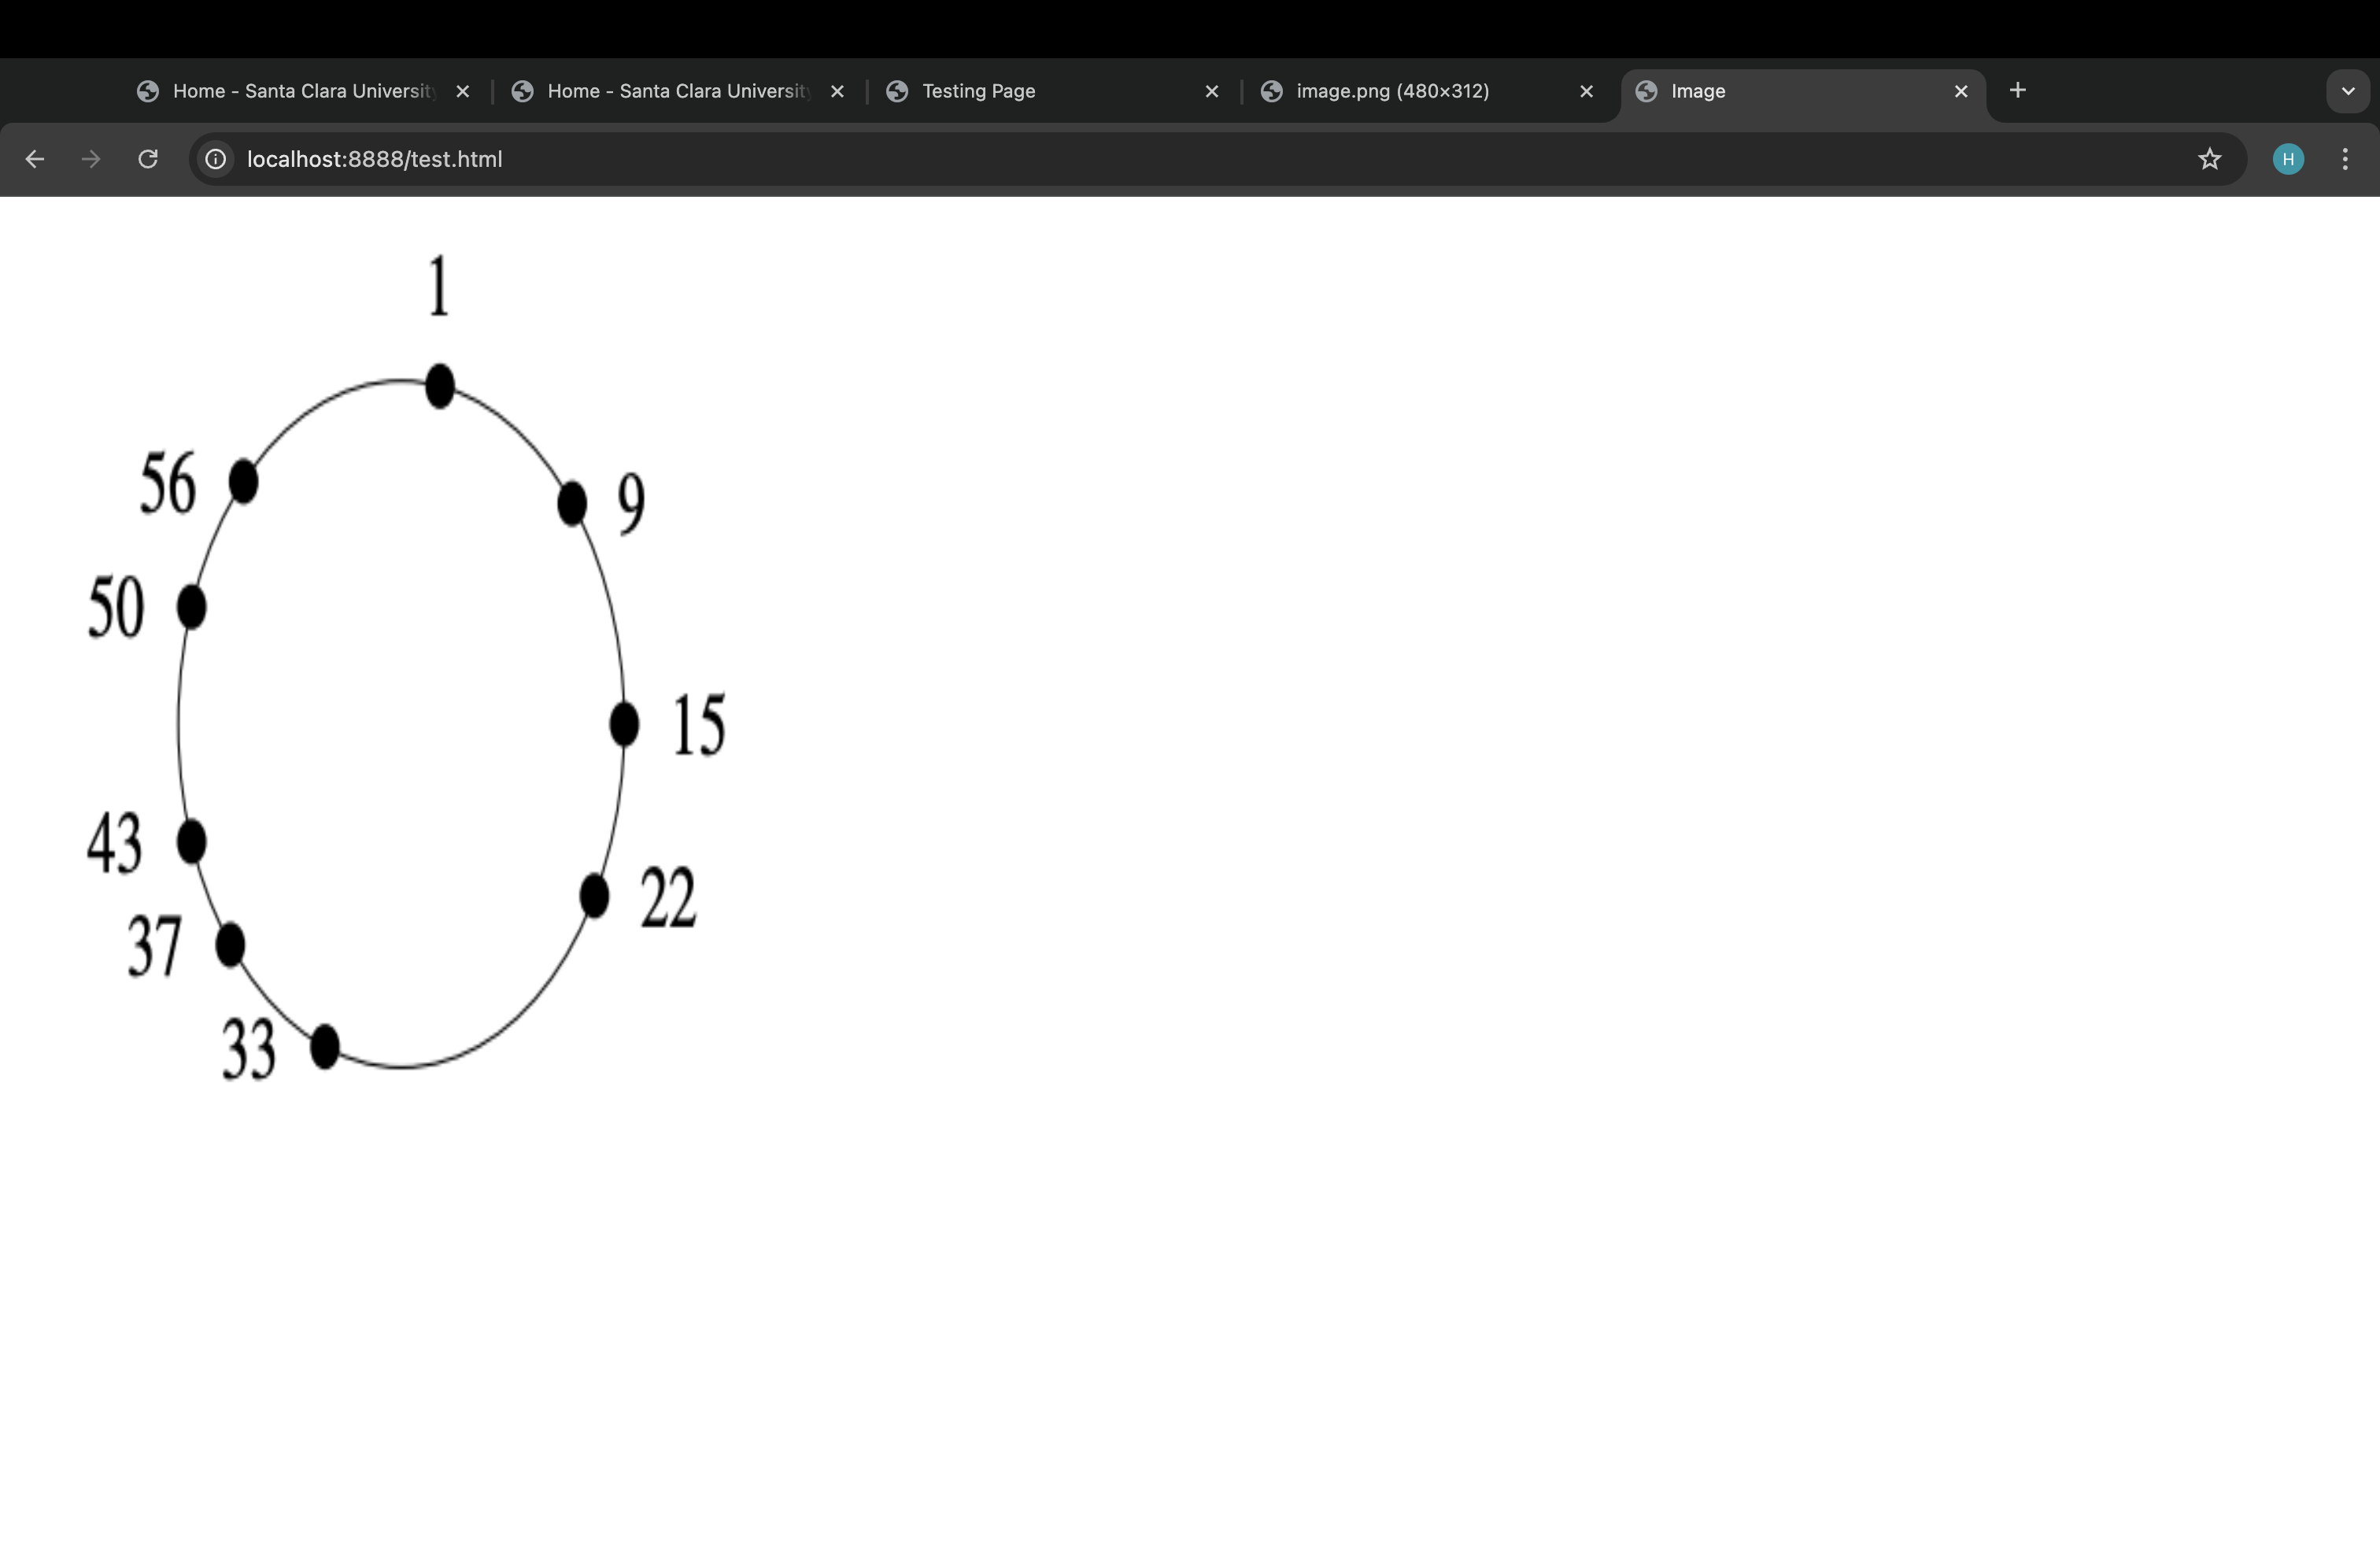
\includegraphics[keepaspectratio]{/outputs/pagewithimage.png}}
- The \texttt{info.html} page provides information and examples of
images being served by the server to test media requests.

\subsubsection{5. Image of Directly Loading an
Image}\label{image-of-directly-loading-an-image}

\pandocbounded{\includegraphics[keepaspectratio]{/outputs/directimage.png}}
- This image shows the browser directly loading an image by accessing
its specific path (\texttt{http://localhost:8000/assets/image.png}).

\subsubsection{\texorpdfstring{6. Image for Loading
\texttt{sample.txt}}{6. Image for Loading sample.txt}}\label{image-for-loading-sample.txt}

\pandocbounded{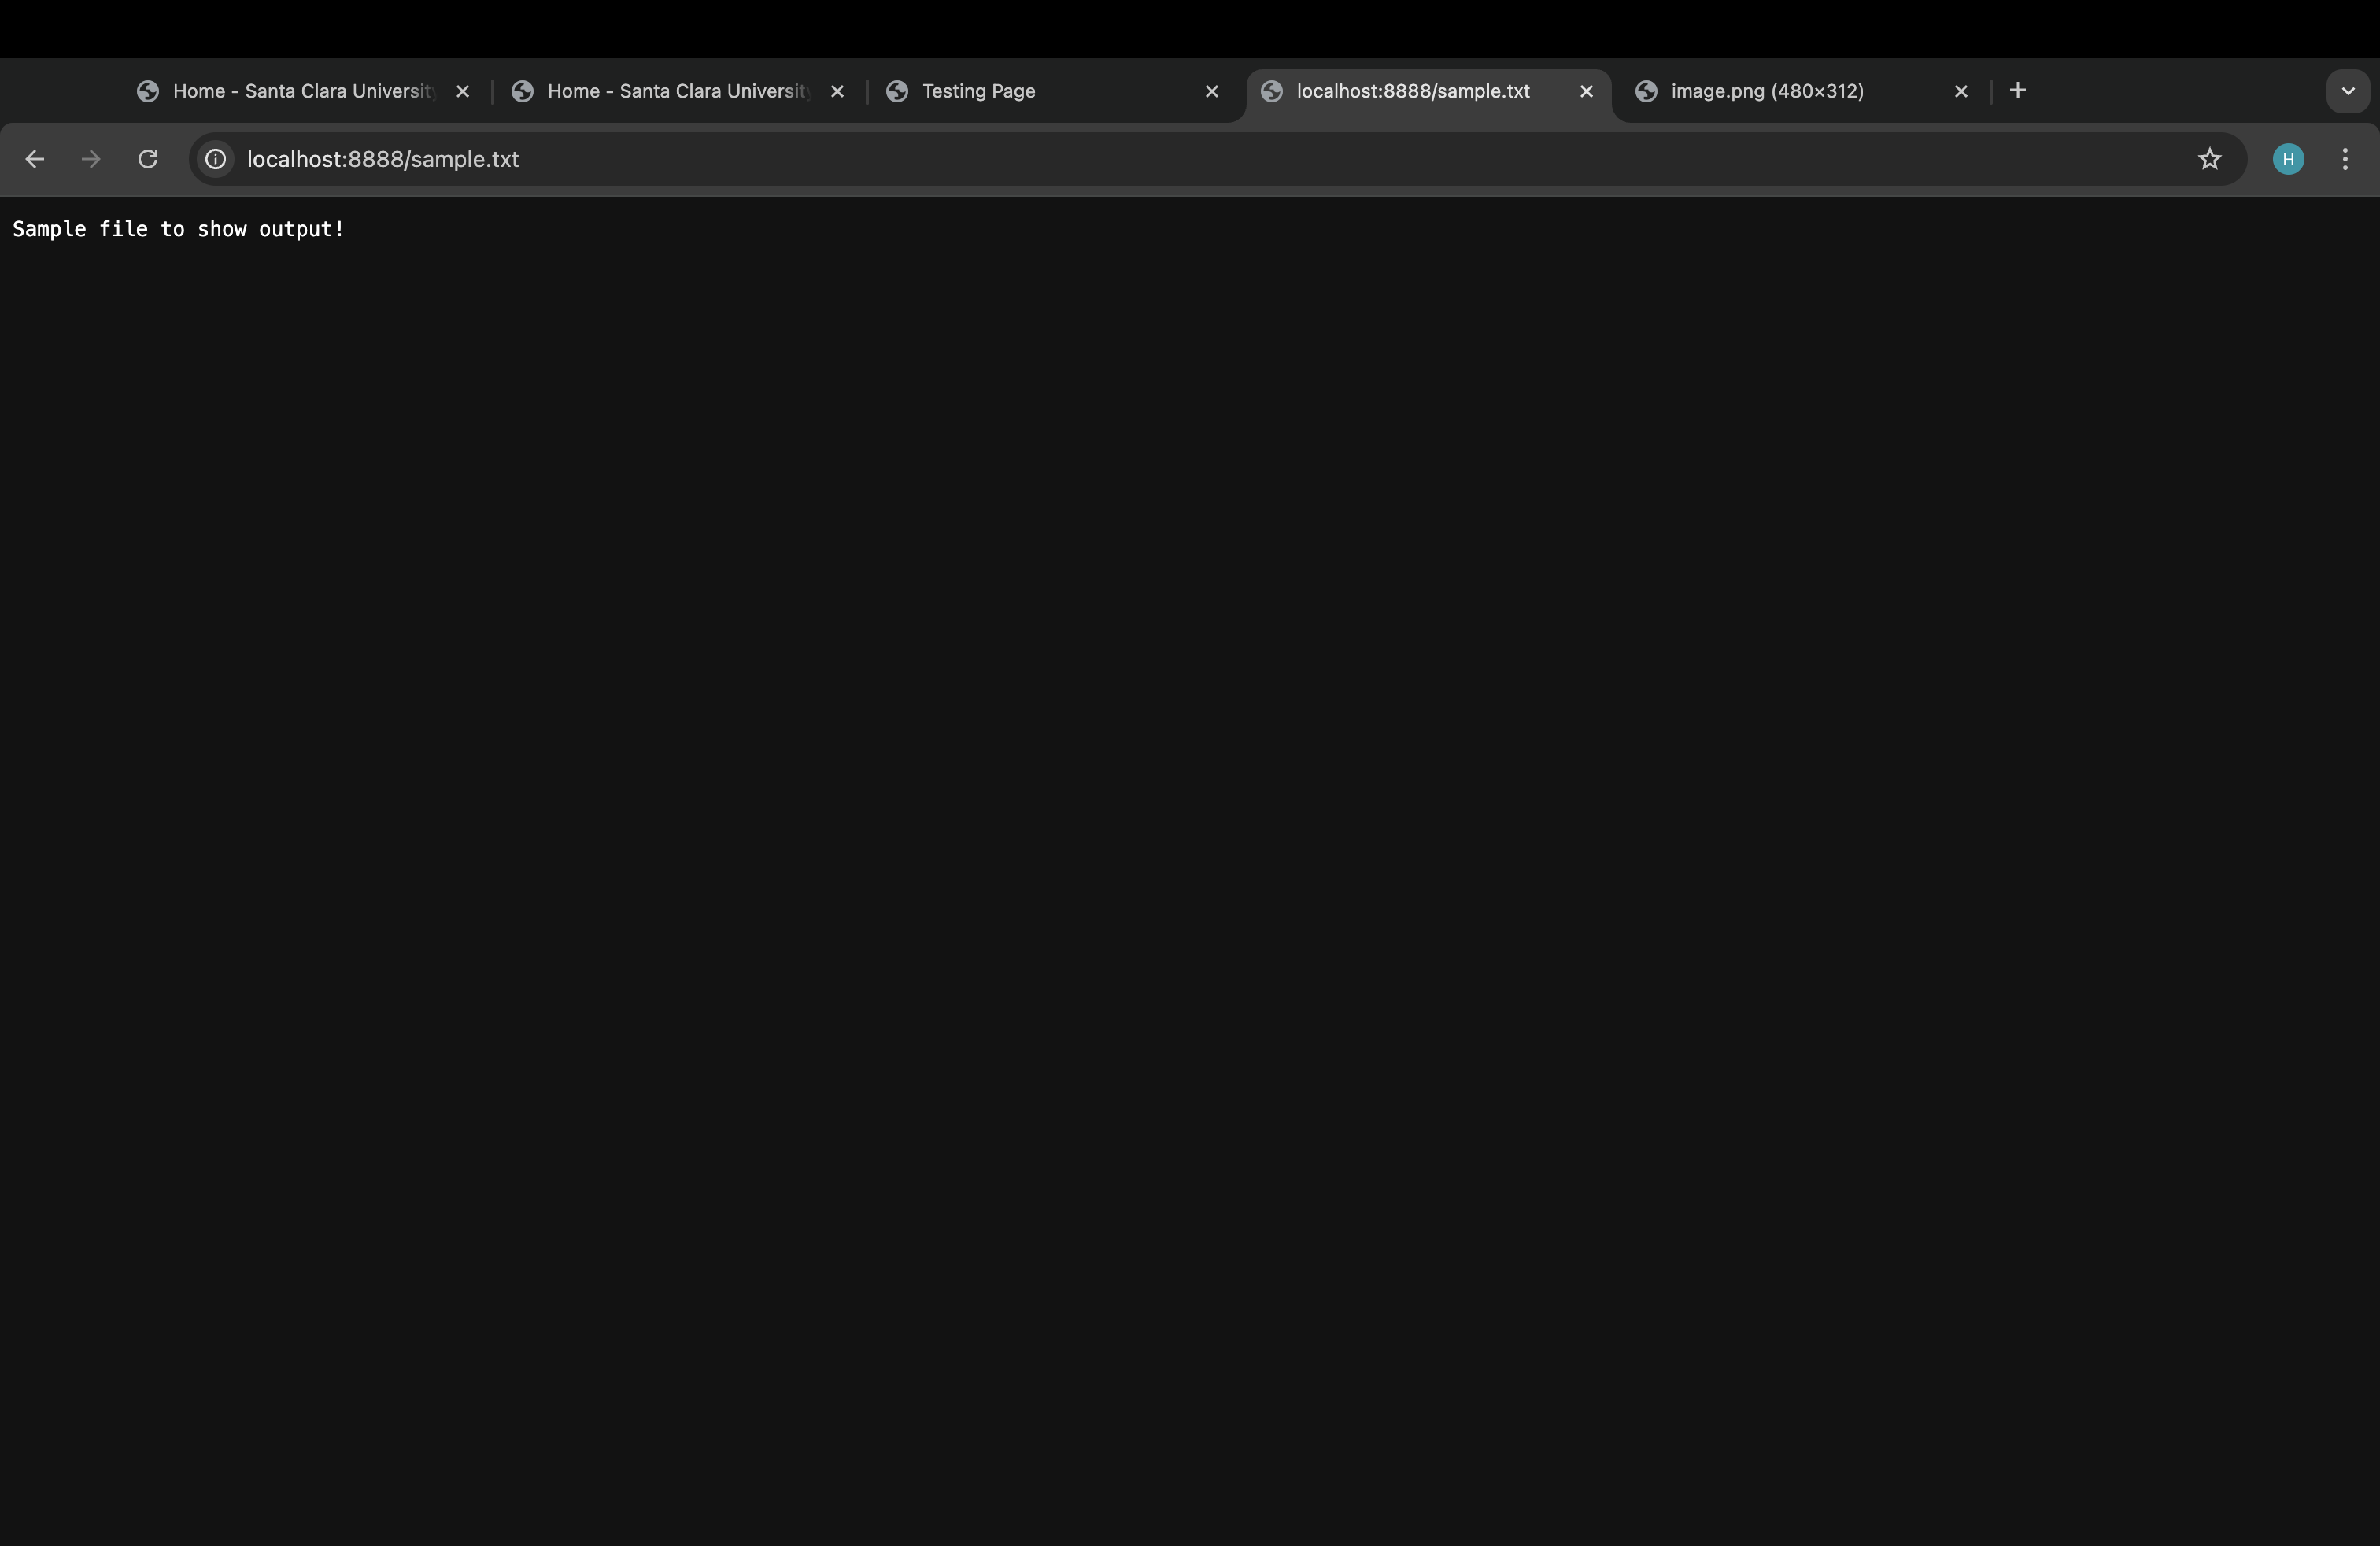
\includegraphics[keepaspectratio]{/outputs/sampletext.png}}
- The \texttt{sample.txt} file is served directly, demonstrating how the
server handles text files with the appropriate \texttt{Content-Type}
header.

\subsubsection{7. Image for Forbidden
Access}\label{image-for-forbidden-access}

\pandocbounded{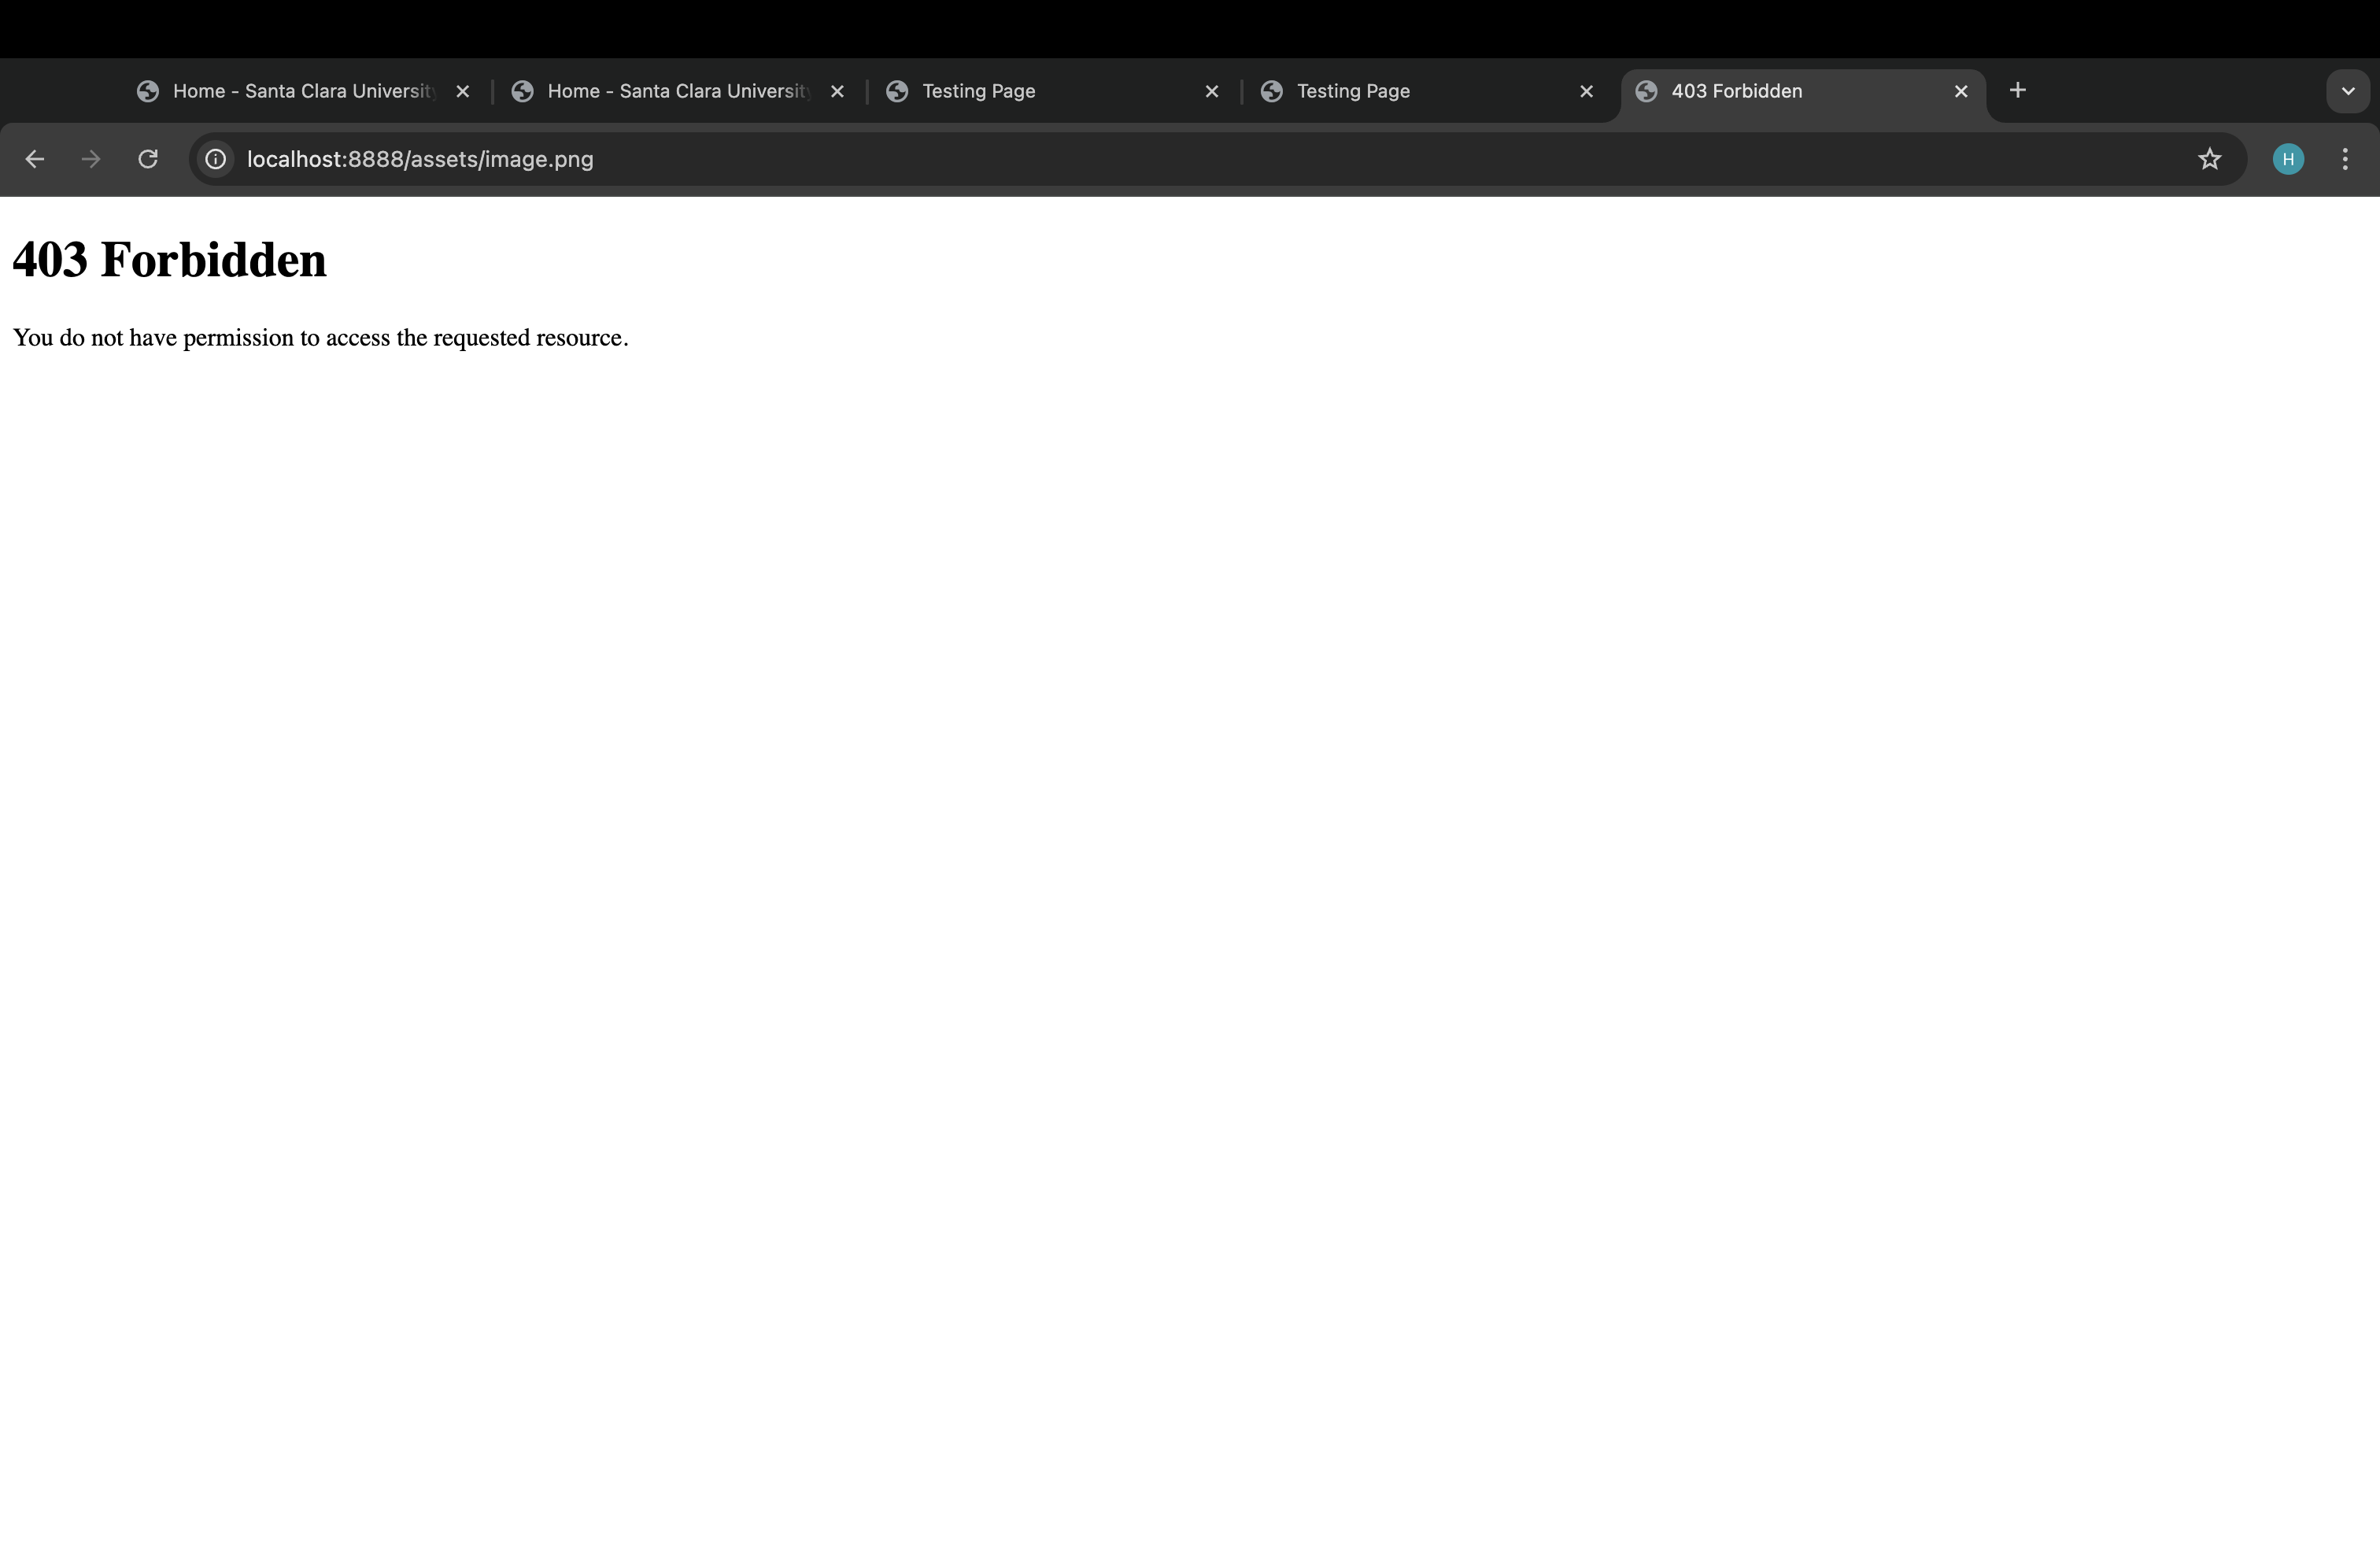
\includegraphics[keepaspectratio]{/outputs/forbidden.png}}
- This image shows the \texttt{403.html} page, which appears when trying
to access a file with insufficient permissions.

\subsubsection{8. Image of Invalid Path}\label{image-of-invalid-path}

\pandocbounded{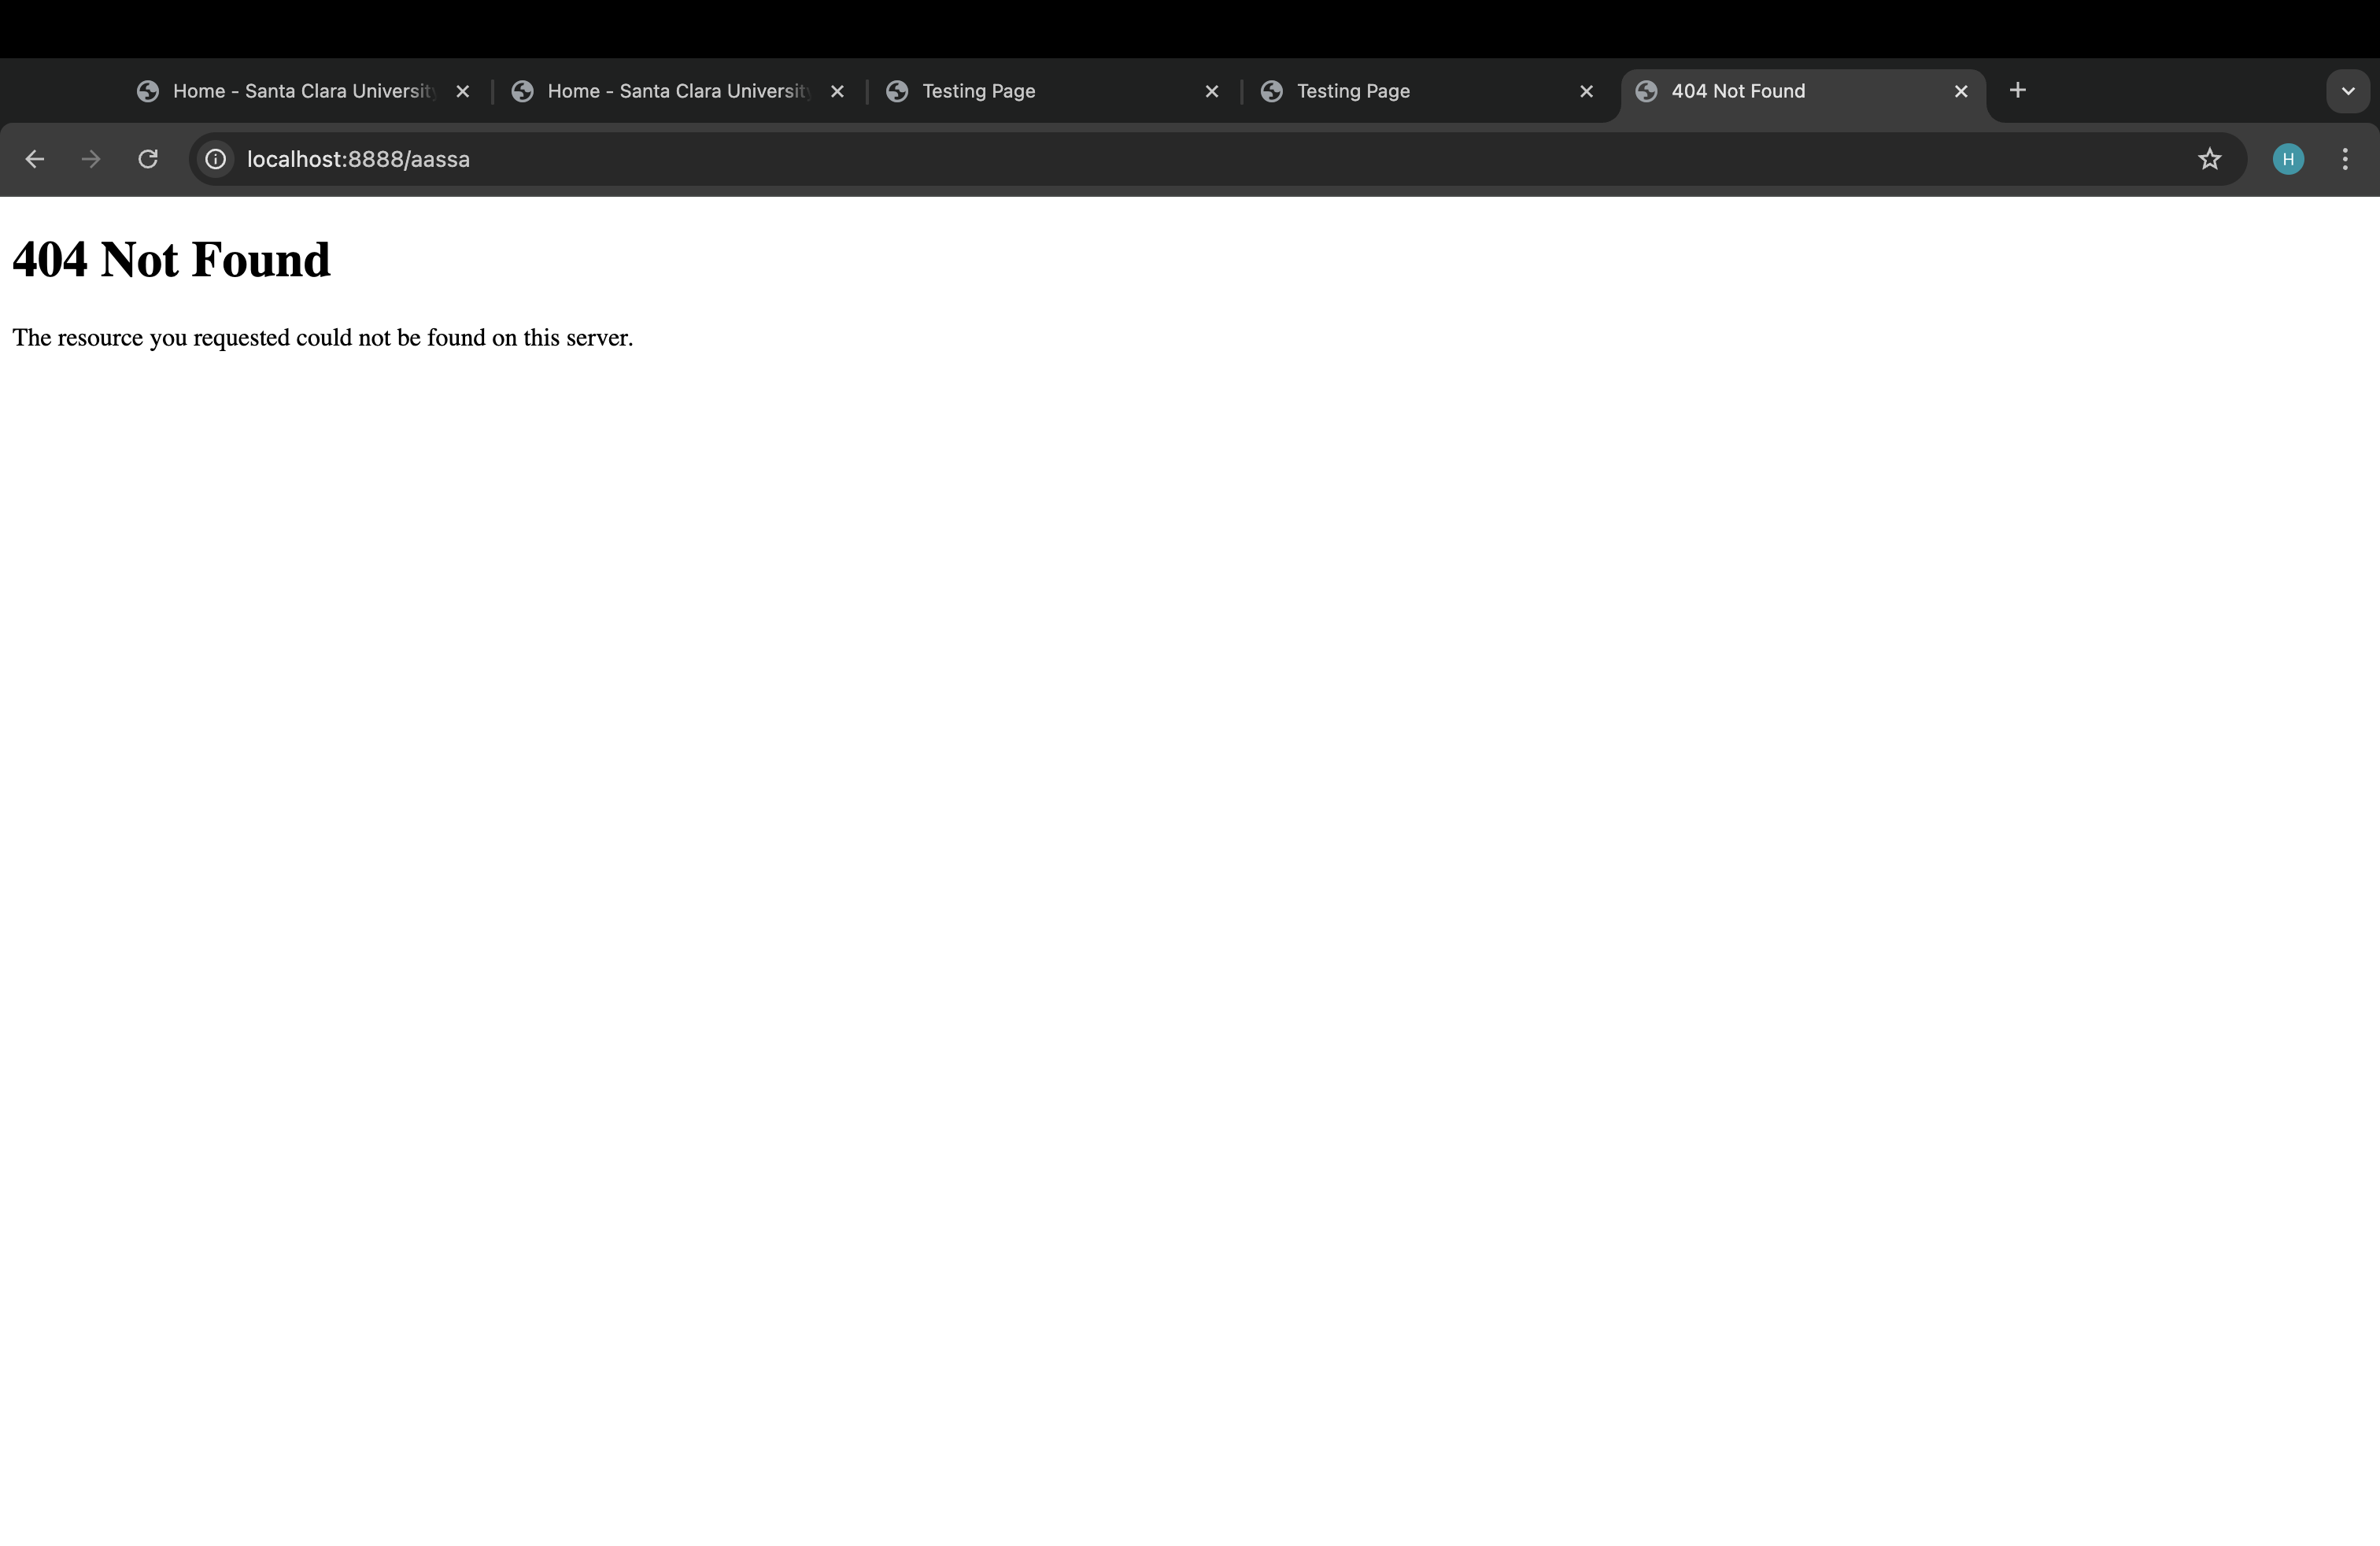
\includegraphics[keepaspectratio]{/outputs/invalidpath.png}}
- When a non-existent path is requested, the server returns a
\texttt{500\ Internal\ Server\ Error} page (\texttt{500.html}). This
image shows the error page being served.

\subsubsection{9. Image for Internal Server
Error}\label{image-for-internal-server-error}

\pandocbounded{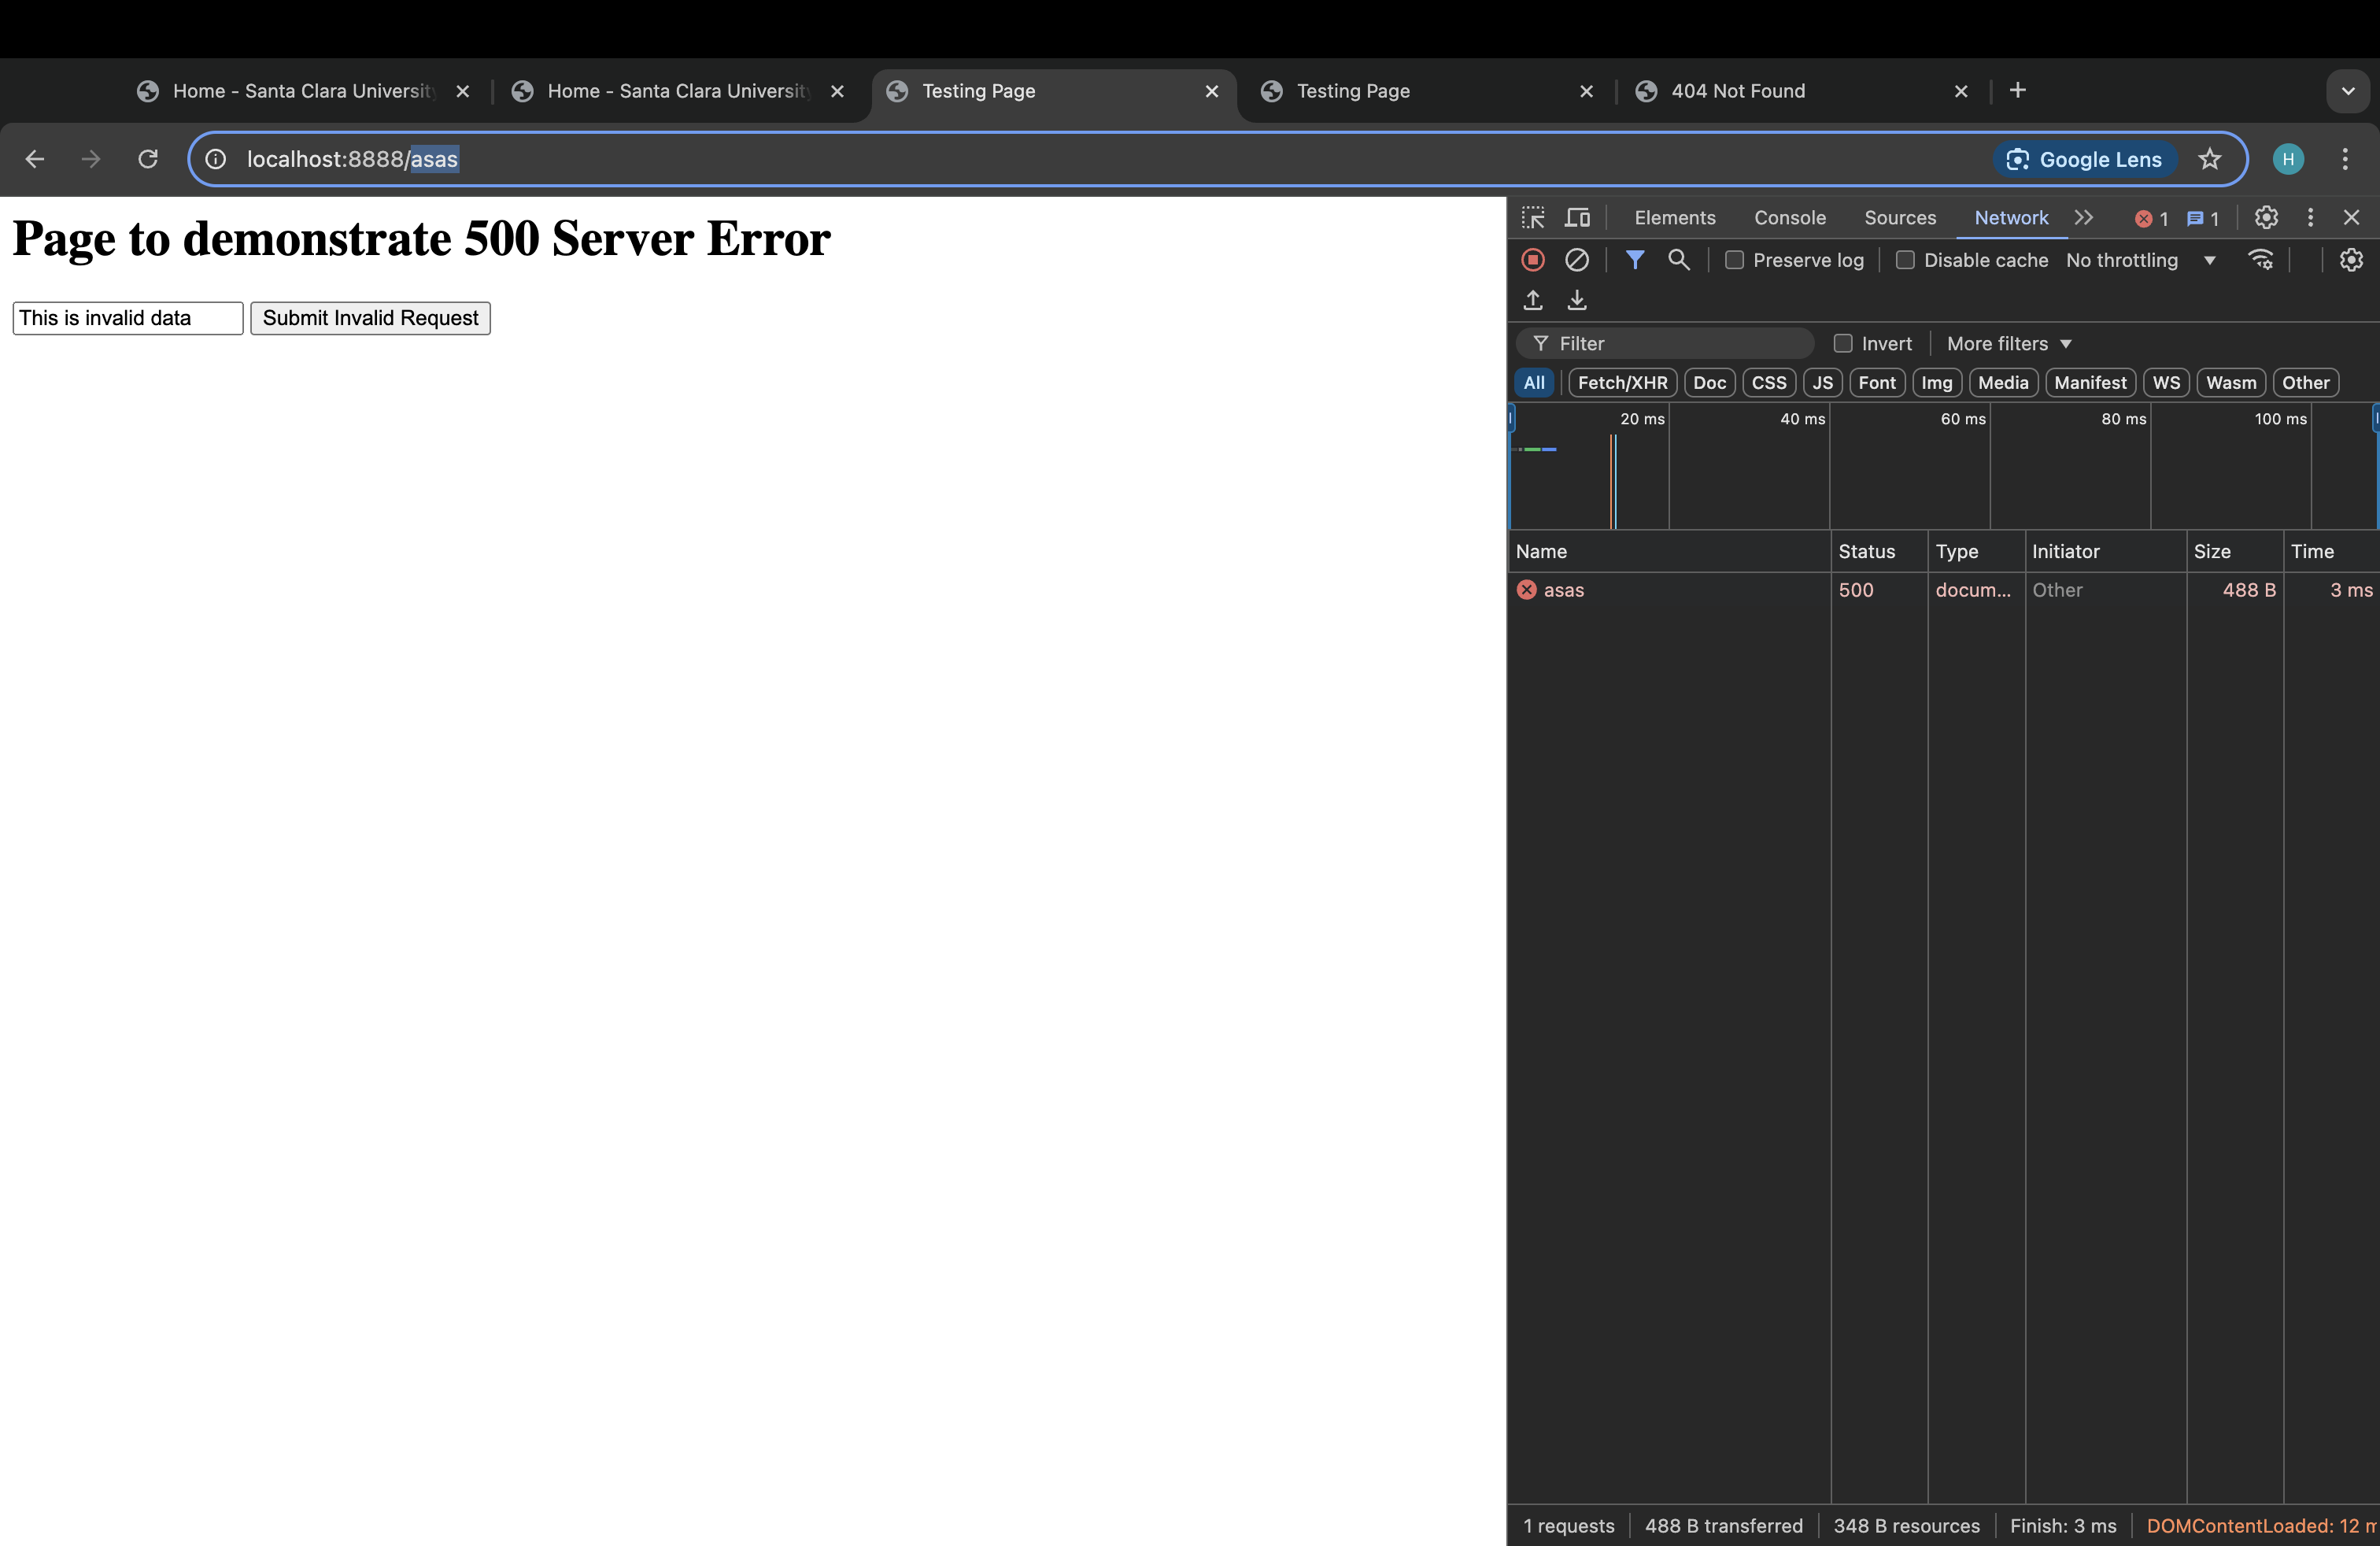
\includegraphics[keepaspectratio]{/outputs/is1.png}}
\pandocbounded{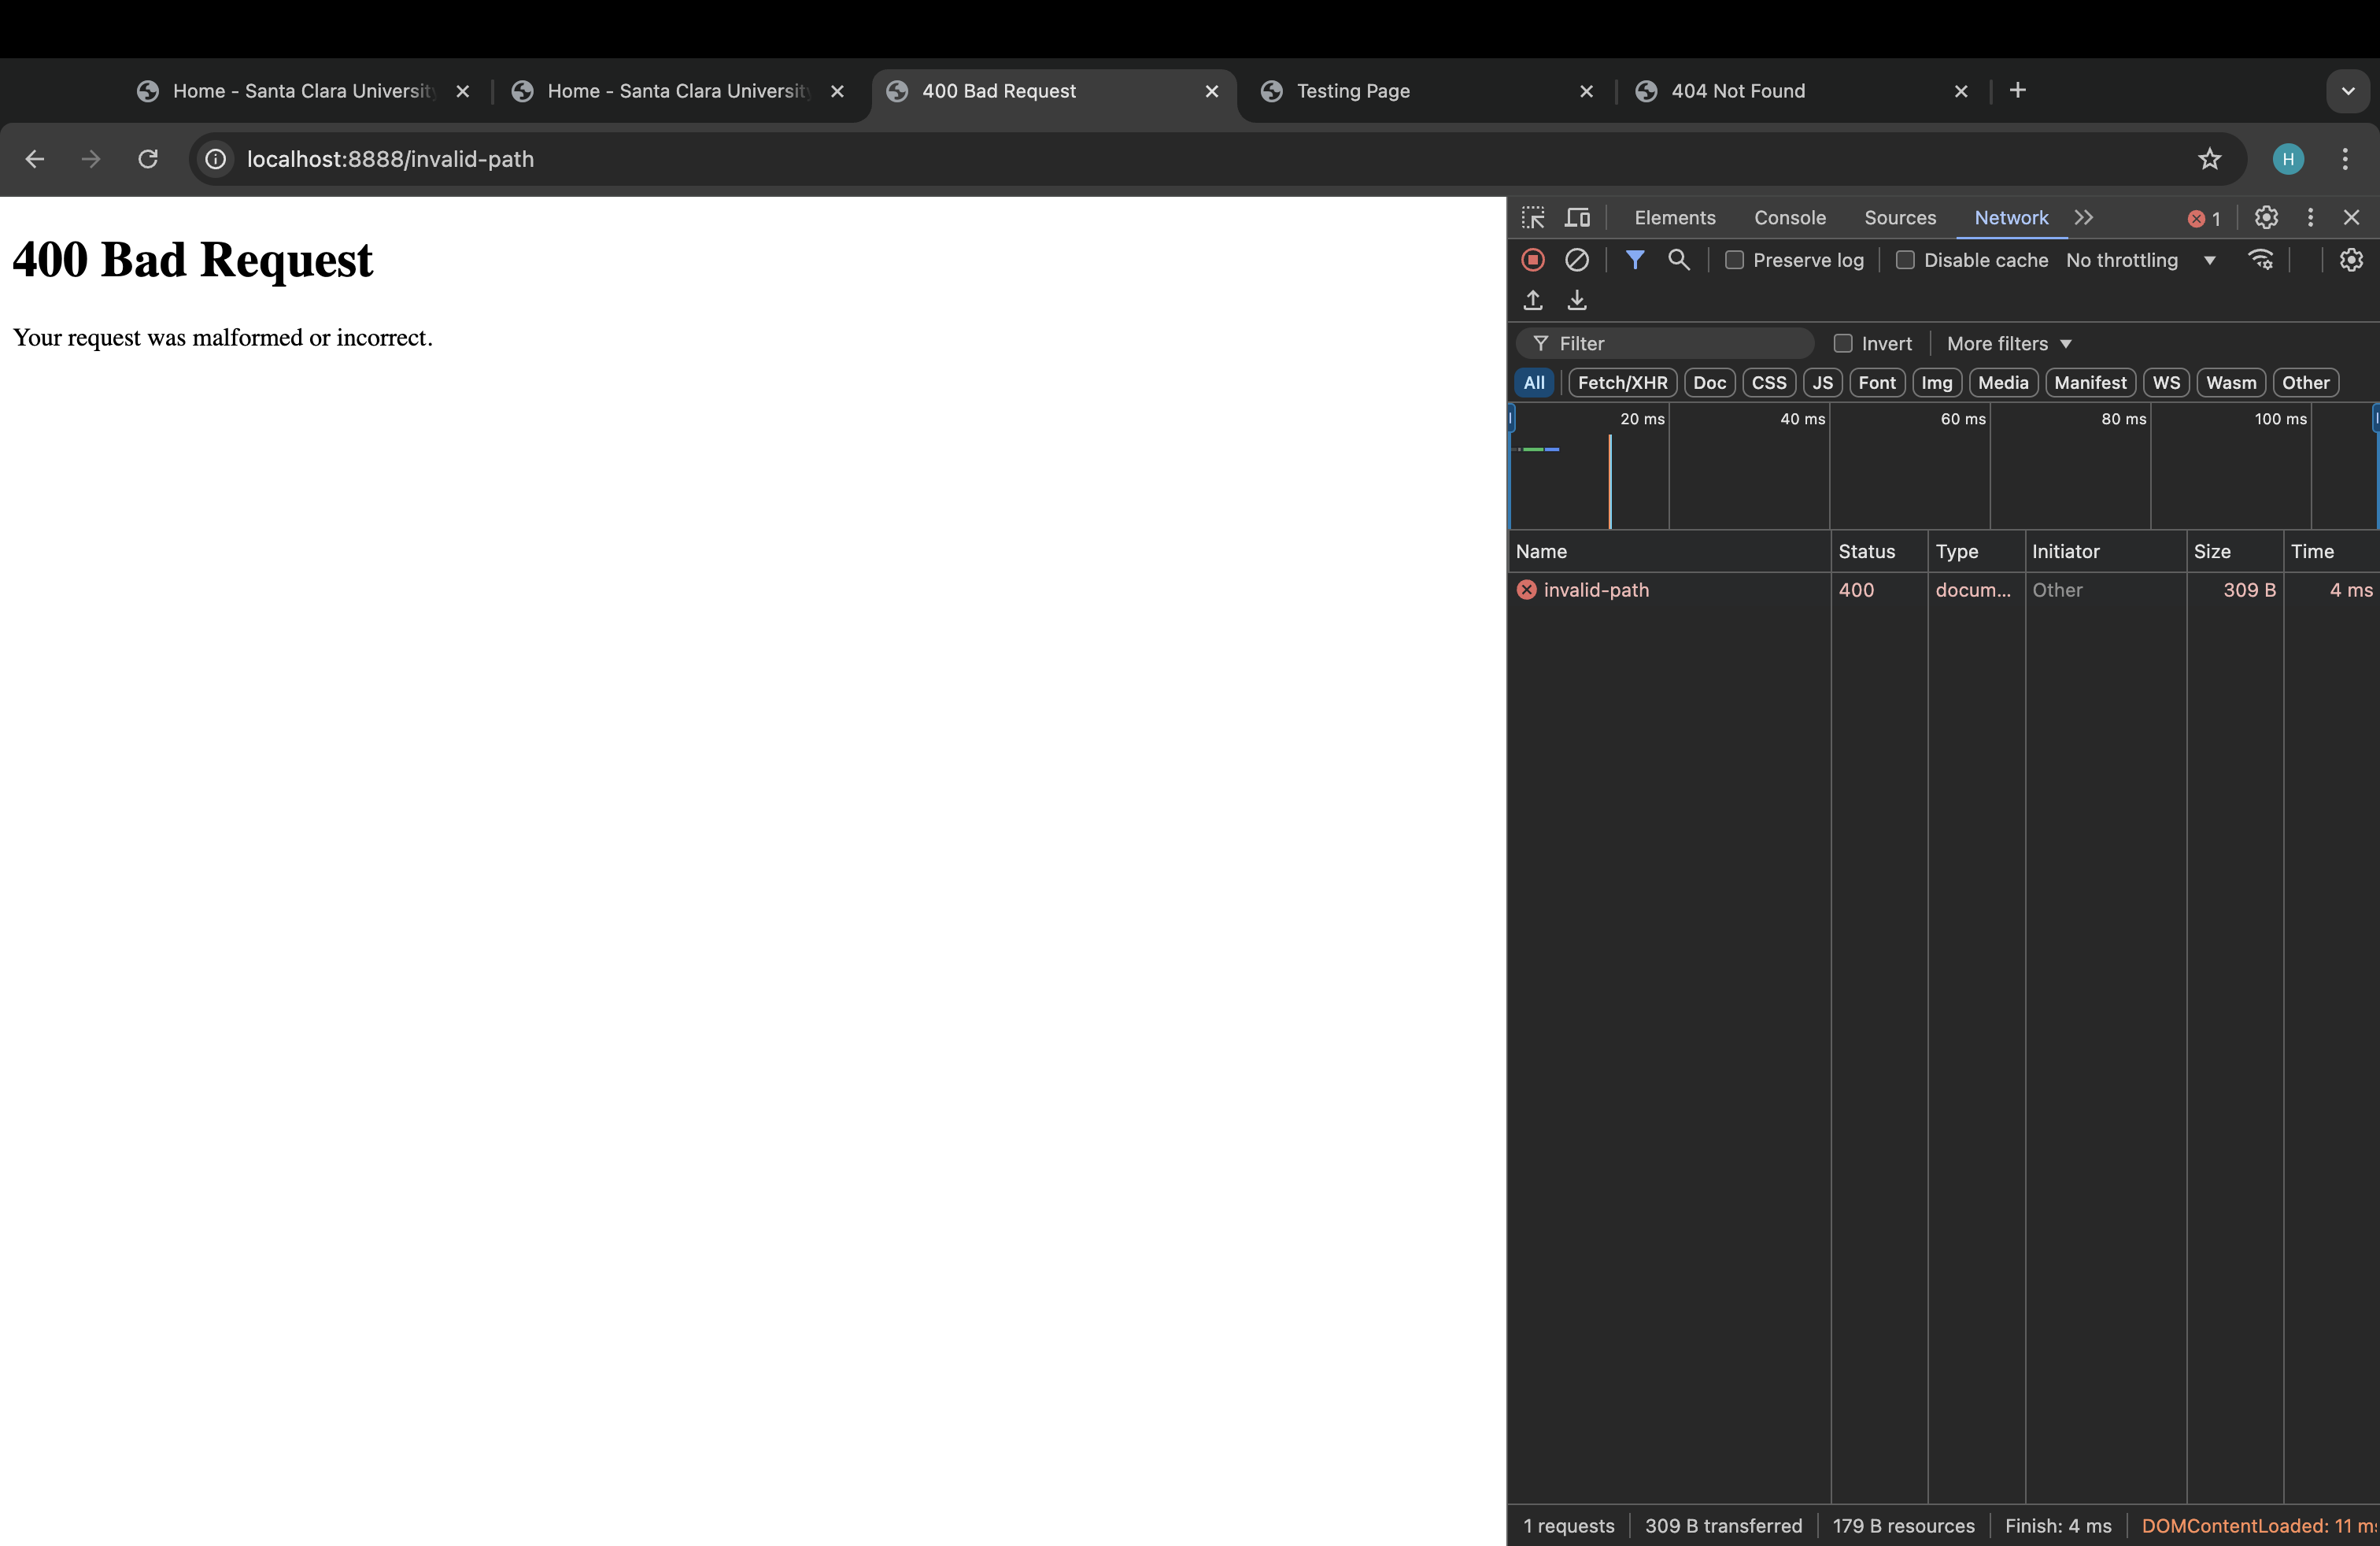
\includegraphics[keepaspectratio]{/outputs/is2.png}} -
Similar to the previous error page, this demonstrates another case where
the server returns an internal server error.

\subsubsection{10. Image to Show Headers}\label{image-to-show-headers}

\pandocbounded{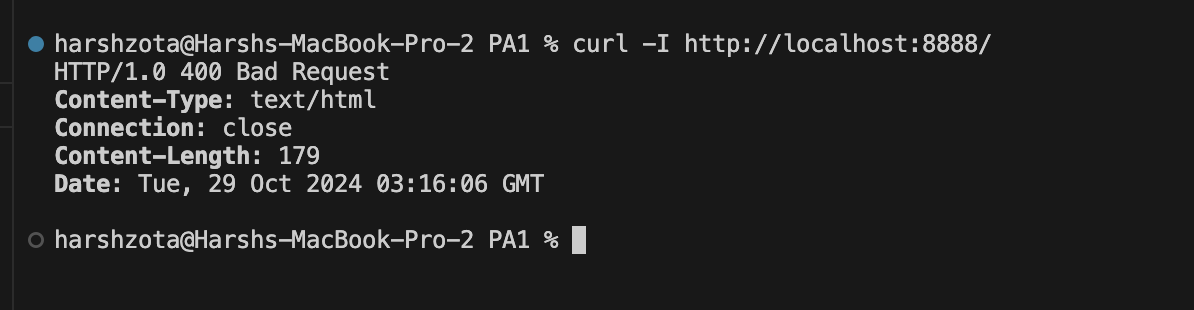
\includegraphics[keepaspectratio]{/outputs/headers.png}}
- This image is taken from browser developer tools, showcasing the HTTP
headers sent by the server, including \texttt{Content-Type},
\texttt{Content-Length}, and connection management.
